%!TeX program = xelatex
%Do not change
\documentclass[12pt, oneside]{article}
\usepackage{amssymb,amsmath}
\usepackage[margin=1in]{geometry}
\usepackage{textpos}
\usepackage{float}
\usepackage{booktabs}
%\usepackage{color}
\usepackage{graphicx}
\usepackage[inter-unit-product =\cdot]{siunitx}
\let\DeclareUSUnit\DeclareSIUnit
\let\US\SI
\DeclareUSUnit\inch{in}
\DeclareUSUnit\foot{ft}
\DeclareUSUnit\mile{mi}
\DeclareUSUnit\foot{ft}
\DeclareUSUnit\slug{slug}
\DeclareUSUnit\pound{lb}
\DeclareUSUnit\psi{psi}
\DeclareUSUnit\Msi{Msi}
\DeclareUSUnit\ksi{ksi}

%\usepackage{tikz}
%\usetikzlibrary{positioning}
%\usepackage{tikz-3dplot}
%\usepackage{pgfopts}
%\usepackage{wasysym}
%\usepackage{stanli}

% You may add the packages you need here
\begin{document}

%TODO change numbers in problems
\begin{textblock*}{4cm}(-1.7cm,-2.3cm)
\noindent {\scriptsize AE333 Spring 2021}
\end{textblock*}

%Do not modify other than putting your name where stated
\begin{textblock*}{8cm}(12.5cm,-1cm)
\noindent {Name: }
\end{textblock*}
%Do not modify other than typing your acknowledgement where stated
\begin{textblock*}{13.5cm}(-1.7cm,-1.8cm)
%\noindent \textit{\footnotesize Acknowledgement: Your acknowledgement for collaboration and other sources goes here. }
\end{textblock*}

\vspace{1cm}

%Do not modify other than typing the homework number after #
\begin{center}
\textbf{\Large Homework 3}

\textbf{Due 8 Mar 2021}
\end{center}

\begin{enumerate}
	\item %F4-3
		The $\SI{30}{mm}$ diameter steel rod is subjected to the loading shown.
		Find the displacement at $C$.
		\begin{figure}[H]
			\centering
			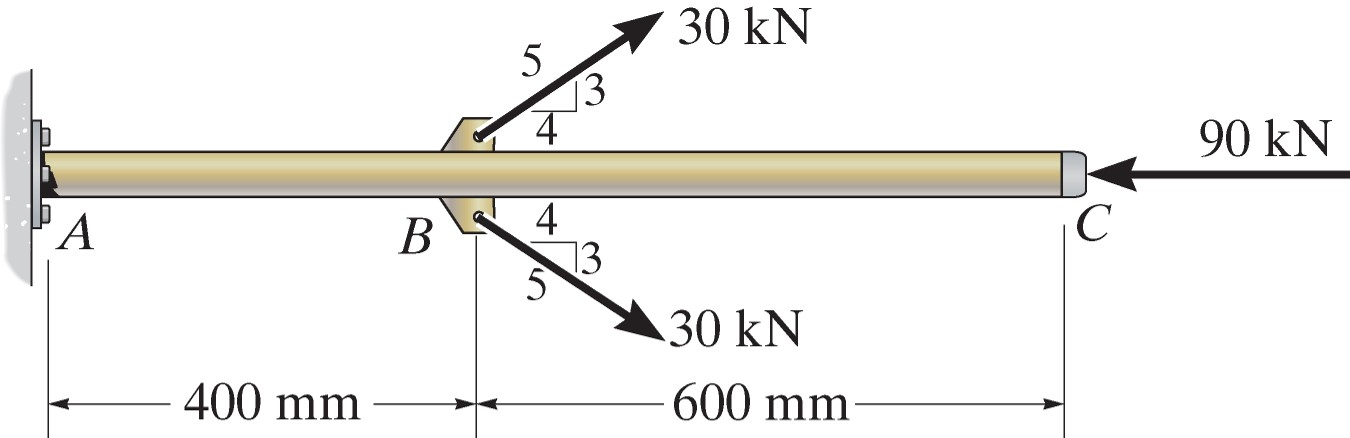
\includegraphics[width=0.8\linewidth]{f4-3}
		\end{figure}

	\item %4-11
		The load is supported by four stainless steel wires that are connected to rigid members $AB$ and $DC$.
		Determine the vertical displacement of the $\US{500}{lb}$ load if each wire has a cross-sectional area of $\US{.035}{in^2}$.
		\begin{figure}[H]
			\centering
			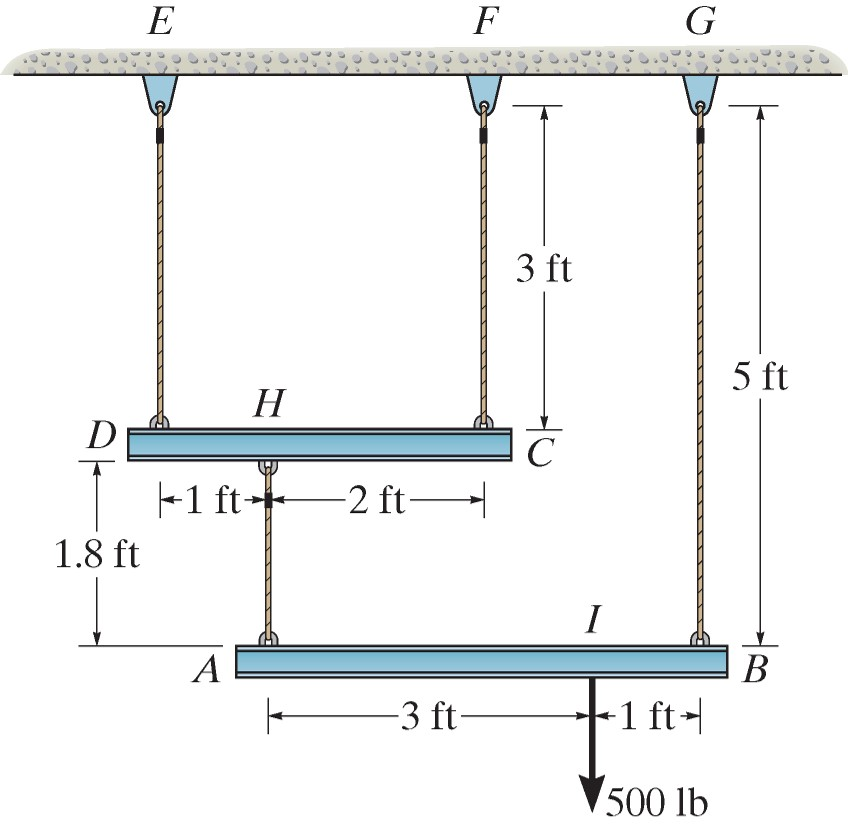
\includegraphics[width=0.5\linewidth]{4-11}
		\end{figure}
		\newpage

	\item %4-32
		The column shown is constructed from concrete with A992 steel rebar.
		If the column is subjected to an axial force of $\US{200}{kip}$, find the required rod diameter such that 60\% of the axial force is carried by the concrete.
		\begin{figure}[H]
			\centering
			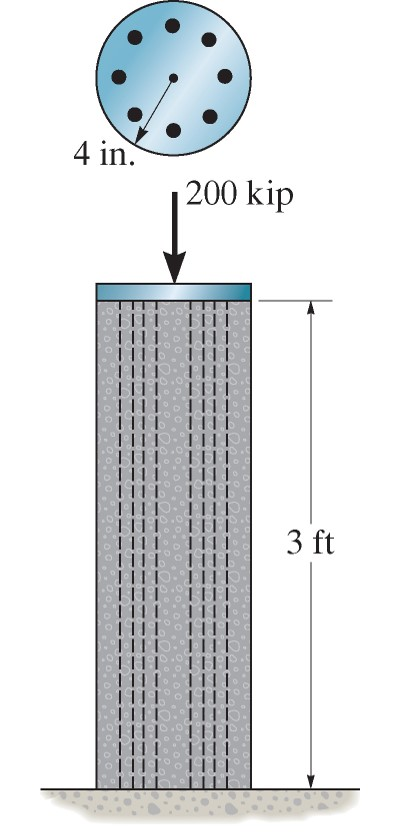
\includegraphics[width=0.25\linewidth]{4-32}
		\end{figure}
	
	\item %4-59
		The post is made from 2024 aluminum and has a diameter of $\SI{50}{mm}$.
		It is fixed at $A$ and $B$ and has a coiled spring attached to a rigid collar at $C$.
		If the spring is initially uncompressed, find the compression in the spring when a load of $P = \SI{75}{kN}$ is applied to the collar.
		\begin{figure}[H]
			\centering
			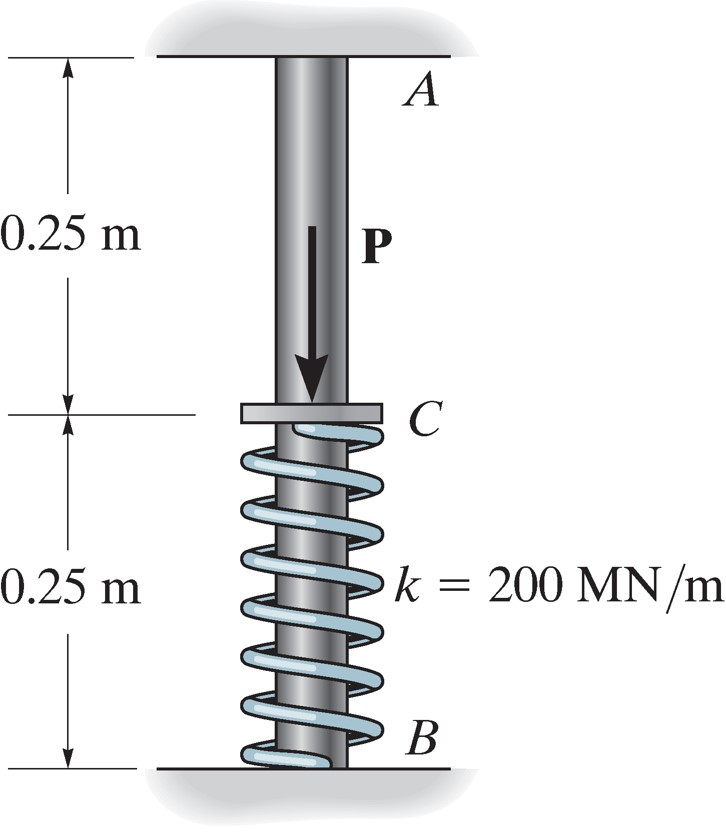
\includegraphics[width=0.45\linewidth]{4-59}
		\end{figure}

	\item %4-69
		The assembly has shown fits snugly with no internal force at $70 ^\circ F$.
		Find the average normal stress in each material when the temperature is raised to $200 ^\circ F$.
		\begin{figure}[H]
			\centering
			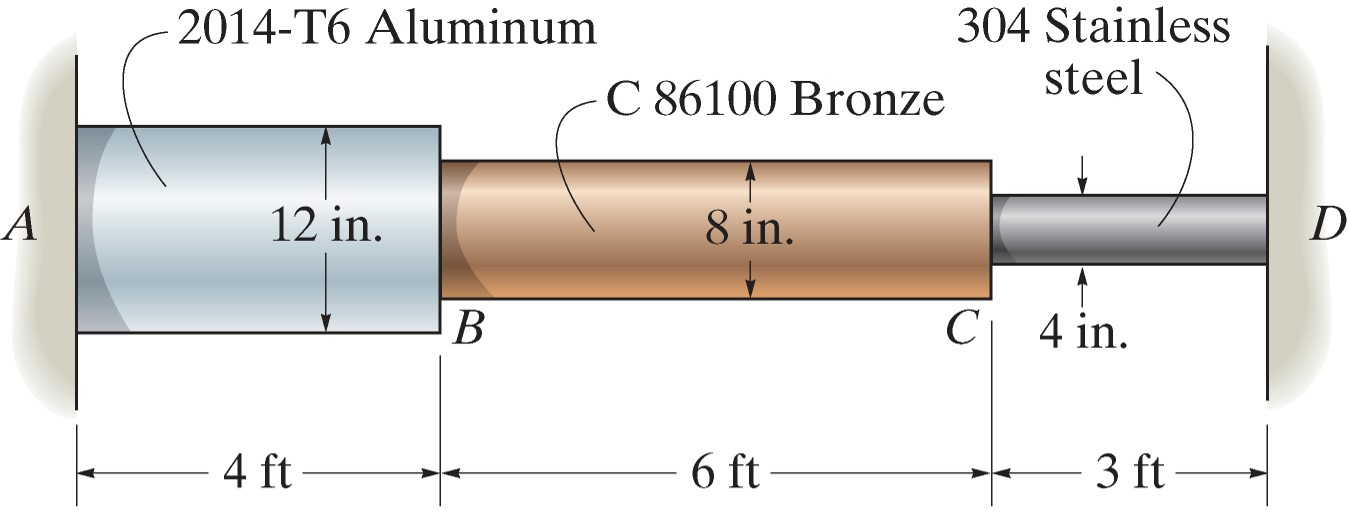
\includegraphics[width=0.8\linewidth]{4-69}
		\end{figure}

	\item %4-70
		The rod shown is made from aluminum and has a diameter of $\US{0.25}{in}$.
		If the rod is $\US{4}{ft}$ long when the springs are compressed $\US{0.5}{in}$ and the temperature of the rod is $40 ^\circ F$, find the force in the rod when the temperature is $150 ^\circ F$.
		\begin{figure}[H]
			\centering
			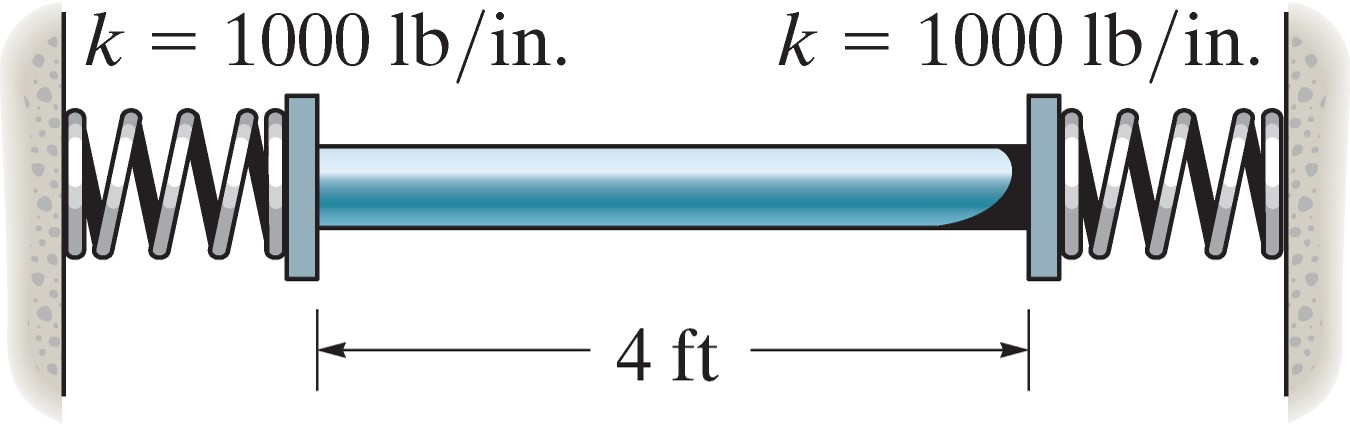
\includegraphics[width=0.8\linewidth]{4-70}
		\end{figure}
		\newpage

	\item %4-76
		The device shown is used to measure temperature.
		Bars $AB$ and $CD$ are made of tungsten ($\alpha = 4.5 \times 10^{-6} \text{ } ^\circ C^{-1}$) and aluminum ($\alpha = 23 \times 10^{-6} \text{ } ^\circ C^{-1}$), respectively.
		At room temperature ($20^\circ C$) the rigid bar $AE$ is horizontal.
		Find the vertical displacement of the pointer when the temperature is $200 ^\circ C$.
		\begin{figure}[H]
			\centering
			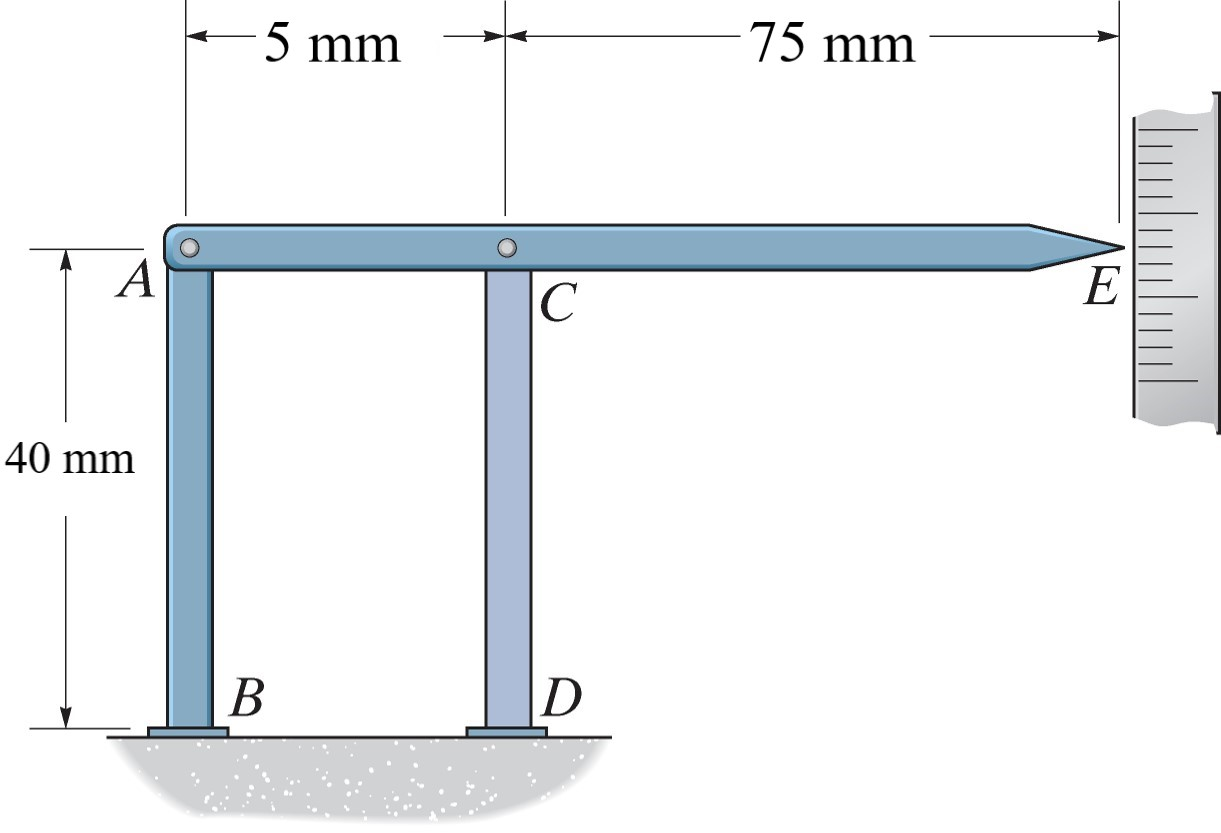
\includegraphics[width=0.8\linewidth]{4-76}
		\end{figure}

\end{enumerate}
\end{document}
